\documentclass[runningheads]{llncs}
\usepackage[utf8]{inputenc}
\usepackage[T1]{fontenc}
\usepackage{geometry}
\usepackage{array}
\usepackage{booktabs}
\usepackage{longtable}
\usepackage{hyperref}
\usepackage{xcolor}
\usepackage{listings}
\usepackage{amsmath}
\usepackage{algorithmicx}
\usepackage{amssymb}
\usepackage{graphicx}
\usepackage{tabularx}
\usepackage{algorithm}
\usepackage{algpseudocode}
\usepackage{tikz}
\usepackage{pgfplots}
\usetikzlibrary{positioning}
\pgfplotsset{compat=1.18}

\geometry{margin=2.5cm}
\hypersetup{
    colorlinks=true,
    linkcolor=blue,
    urlcolor=blue
}

\lstdefinestyle{bashstyle}{
    basicstyle=\ttfamily\small,
    breaklines=true,
    frame=single,
    backgroundcolor=\color{gray!8},
    columns=fullflexible
}

\title{Implementation and Optimization of the HQC Decoder on NPU-Integrated Devices}
\author{}
\date{}

\begin{document}

\maketitle

\begin{abstract}
    \input{abstract_intro/Abstract}    
\end{abstract}

\section{Introduction}
\input{abstract_intro/Intro}

\section{Background}

\input{background/Codes}

\subsection{NPU}

\input{background/NPU}

\section{Proposed algorithms}
\input{methodology/Proposed_algorithm}

\subsection{RM decoding}
\input{methodology/RM_code}
\subsection{RS decoding}
\input{methodology/RS_code}

 
\section{Benchmark}

\subsection{Experimental setting}

We evaluate the HQC-128 decode path with the same corpus used by the
implementation tests: 16 deterministic decode fixtures per iteration.  All
reported runs pass the correctness check.  Simulator measurements use
\texttt{hexagon-sim} and report Pcycles, while real-device measurements use
host-observed wall-clock latency from the benchmark process.

For the simulator, the full-decode estimate subtracts the fixed cost of the
1-iteration run from the 10-iteration run:
\[
  \text{Pcycles/decode} =
  \frac{\text{Pcycles}_{10\text{ iters}}-\text{Pcycles}_{1\text{ iter}}}
       {9 \times 16}.
\]
For isolated substages, the same method is applied to the substage operation
count:
\[
  \text{Pcycles/op} =
  \frac{\text{Pcycles}_{10\text{ iters}}-\text{Pcycles}_{1\text{ iter}}}
       {\text{ops}_{10\text{ iters}}-\text{ops}_{1\text{ iter}}}.
\]
RM substages are converted to per-decode cost by multiplying the per-block
cost by \(46\), the number of Reed--Muller blocks in HQC-128.

\subsection{Simulation results}

The simulator benchmark compares three code paths.  \texttt{scalar} is the
portable Hexagon baseline.  \texttt{default CT} is the HVX intrinsic path with
fixed-flow RS roots and arithmetic RM/GF code.  \texttt{fastest non-CT} is a
benchmark-only path using side-channel-relaxed RS control flow and
data-dependent GF/RM lookup tables.

\begin{table}[t]
\centering
\caption{Full-decode simulator result on the 16-fixture corpus.}
\label{tab:sim-full-derived}
\small
\begin{tabular}{lrrr}
\toprule
Variant & Pcycles/decode & Speedup vs. scalar & Reduction vs. scalar \\
\midrule
Scalar & 953,767 & \(1.00\times\) & 0.0\% \\
Default CT & 252,490 & \(3.78\times\) & 73.5\% \\
Fastest non-CT & 58,605 & \(16.27\times\) & 93.9\% \\
\bottomrule
\end{tabular}
\end{table}

\begin{table}[t]
\centering
\caption{Full-decode raw simulator counters.}
\label{tab:sim-full-raw}
\small
\begin{tabular}{lrrrr}
\toprule
Variant & Iters & Fixtures & Total instructions & Total Pcycles \\
\midrule
Scalar & 1 & 16 & 15,658,494 & 17,831,082 \\
Scalar & 10 & 16 & 139,903,064 & 155,173,506 \\
Default CT & 1 & 16 & 5,268,713 & 6,724,140 \\
Default CT & 10 & 16 & 35,464,291 & 43,082,676 \\
Fastest non-CT & 1 & 16 & 3,370,774 & 4,427,013 \\
Fastest non-CT & 10 & 16 & 9,888,738 & 12,866,145 \\
\bottomrule
\end{tabular}
\end{table}

\begin{figure}[t]
\centering
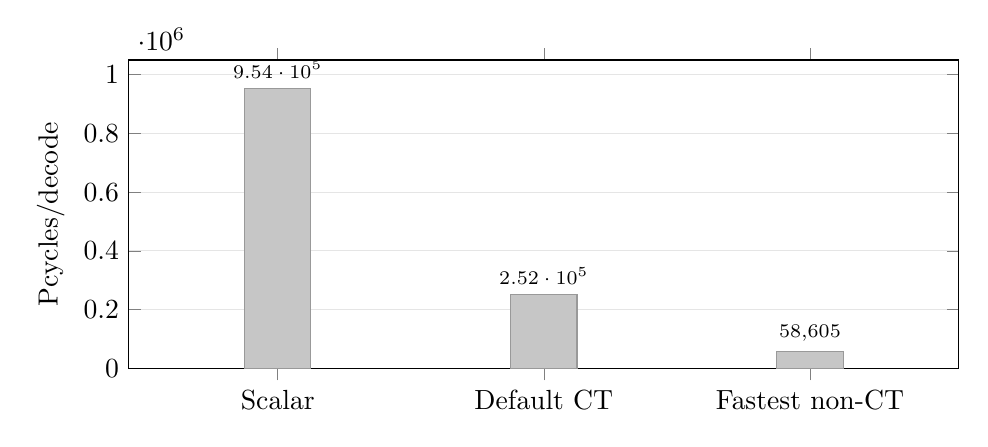
\begin{tikzpicture}
\begin{axis}[
    ybar,
    width=\linewidth,
    height=5.5cm,
    bar width=24pt,
    ymin=0,
    ylabel={Pcycles/decode},
    symbolic x coords={Scalar,Default CT,Fastest non-CT},
    xtick=data,
    nodes near coords,
    nodes near coords align={vertical},
    every node near coord/.append style={font=\scriptsize},
    ymajorgrids=true,
    grid style={gray!20},
    enlarge x limits=0.28,
]
\addplot[fill=gray!45, draw=gray!80] coordinates {
    (Scalar,953767)
    (Default CT,252490)
    (Fastest non-CT,58605)
};
\end{axis}
\end{tikzpicture}
\caption{Full HQC-128 decode cost in the simulator.  Lower is better.}
\label{fig:sim-full-bars}
\end{figure}

\subsection{Substage breakdown}

Figure~\ref{fig:sim-substage-stack} gives a component-level view similar to
the runtime breakdown chart style used in recent HQC optimization work.  The
bars are based on isolated substage measurements, so their sums are not forced
to equal the full-decode benchmark.  Setup cost, cache state, helper
boundaries, and fused paths differ between isolated and end-to-end runs.

\begin{figure}[t]
\centering
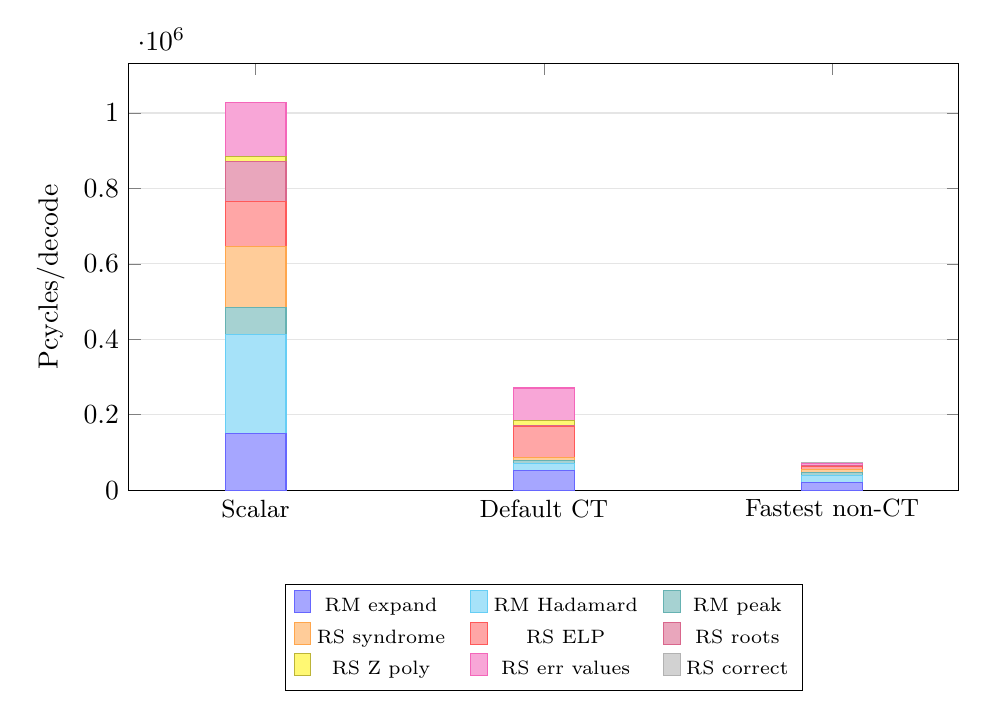
\begin{tikzpicture}
\begin{axis}[
    ybar stacked,
    width=\linewidth,
    height=7.0cm,
    bar width=22pt,
    ymin=0,
    ylabel={Pcycles/decode},
    symbolic x coords={Scalar,Default CT,Fastest non-CT},
    xtick=data,
    x tick label style={font=\small, align=center},
    legend style={
        at={(0.5,-0.22)},
        anchor=north,
        legend columns=3,
        font=\scriptsize,
        /tikz/every even column/.append style={column sep=0.25cm}
    },
    ymajorgrids=true,
    grid style={gray!20},
    enlarge x limits=0.22,
]
\addplot[fill=blue!35, draw=blue!60] coordinates
    {(Scalar,149742) (Default CT,51624) (Fastest non-CT,20988)};
\addlegendentry{RM expand}
\addplot[fill=cyan!35, draw=cyan!60] coordinates
    {(Scalar,263167) (Default CT,18907) (Fastest non-CT,18908)};
\addlegendentry{RM Hadamard}
\addplot[fill=teal!35, draw=teal!60] coordinates
    {(Scalar,71216) (Default CT,8012) (Fastest non-CT,6080)};
\addlegendentry{RM peak}
\addplot[fill=orange!40, draw=orange!70] coordinates
    {(Scalar,162309) (Default CT,8637) (Fastest non-CT,8637)};
\addlegendentry{RS syndrome}
\addplot[fill=red!35, draw=red!65] coordinates
    {(Scalar,119591) (Default CT,81860) (Fastest non-CT,7879)};
\addlegendentry{RS ELP}
\addplot[fill=purple!35, draw=purple!60] coordinates
    {(Scalar,105765) (Default CT,3447) (Fastest non-CT,2132)};
\addlegendentry{RS roots}
\addplot[fill=yellow!55, draw=yellow!70!black] coordinates
    {(Scalar,13044) (Default CT,11146) (Fastest non-CT,1141)};
\addlegendentry{RS Z poly}
\addplot[fill=magenta!35, draw=magenta!60] coordinates
    {(Scalar,143106) (Default CT,87397) (Fastest non-CT,6004)};
\addlegendentry{RS err values}
\addplot[fill=gray!35, draw=gray!60] coordinates
    {(Scalar,439) (Default CT,439) (Fastest non-CT,439)};
\addlegendentry{RS correct}
\end{axis}
\end{tikzpicture}
\caption{Isolated substage cost breakdown from simulator Pcycles.}
\label{fig:sim-substage-stack}
\end{figure}

\begin{table}[t]
\centering
\caption{Dominant isolated substage costs after HVX optimization.}
\label{tab:sim-substage-selected}
\small
\begin{tabular}{lrrr}
\toprule
Substage & Scalar & Default CT & Fastest non-CT \\
\midrule
RM expand/sum & 149,742 & 51,624 & 20,988 \\
RM Hadamard & 263,167 & 18,907 & 18,908 \\
RS syndrome & 162,309 & 8,637 & 8,637 \\
RS ELP & 119,591 & 81,860 & 7,879 \\
RS roots & 105,765 & 3,447 & 2,132 \\
RS error values & 143,106 & 87,397 & 6,004 \\
\bottomrule
\end{tabular}
\end{table}

\subsection{Real-device results}

The real-device benchmarks were run on two Qualcomm platforms.  RB3 Gen 2
uses a QCS6490 Linux system.  QRD8650 is a Snapdragon 8 Gen 3 Android
reference device.  Each main run uses 10,000 iterations, or 160,000 total
decodes.  The cDSP benchmarks make one FastRPC call for the whole decode loop,
so the fixed FastRPC call overhead is amortized in these long runs.

\begin{table}[t]
\centering
\caption{RB3 Gen 2 / QCS6490 Linux decode latency.}
\label{tab:rb3-results}
\small
\begin{tabular}{lrrrr}
\toprule
Variant & us/decode & Throughput & Speedup vs. CPU & Speedup vs. cDSP \\
\midrule
CPU scalar & 106.479 & 9,391.5 & \(1.00\times\) & \(4.55\times\) \\
cDSP scalar & 484.554 & 2,063.8 & \(0.22\times\) & \(1.00\times\) \\
cDSP default CT & 110.908 & 9,016.5 & \(0.96\times\) & \(4.37\times\) \\
cDSP fastest non-CT & 47.495 & 21,054.8 & \(2.24\times\) & \(10.20\times\) \\
\bottomrule
\end{tabular}
\end{table}

\begin{table}[t]
\centering
\caption{QRD8650 / Snapdragon 8 Gen 3 Android decode latency.}
\label{tab:qrd8650-results}
\small
\begin{tabular}{lrrrr}
\toprule
Variant & us/decode & Throughput & Speedup vs. CPU & Speedup vs. cDSP \\
\midrule
CPU scalar & 70.971 & 14,090.3 & \(1.00\times\) & \(5.20\times\) \\
cDSP scalar & 369.007 & 2,710.0 & \(0.19\times\) & \(1.00\times\) \\
cDSP default CT & 86.633 & 11,542.9 & \(0.82\times\) & \(4.26\times\) \\
cDSP fastest non-CT & 37.456 & 26,698.0 & \(1.89\times\) & \(9.85\times\) \\
\bottomrule
\end{tabular}
\end{table}

\begin{figure}[t]
\centering
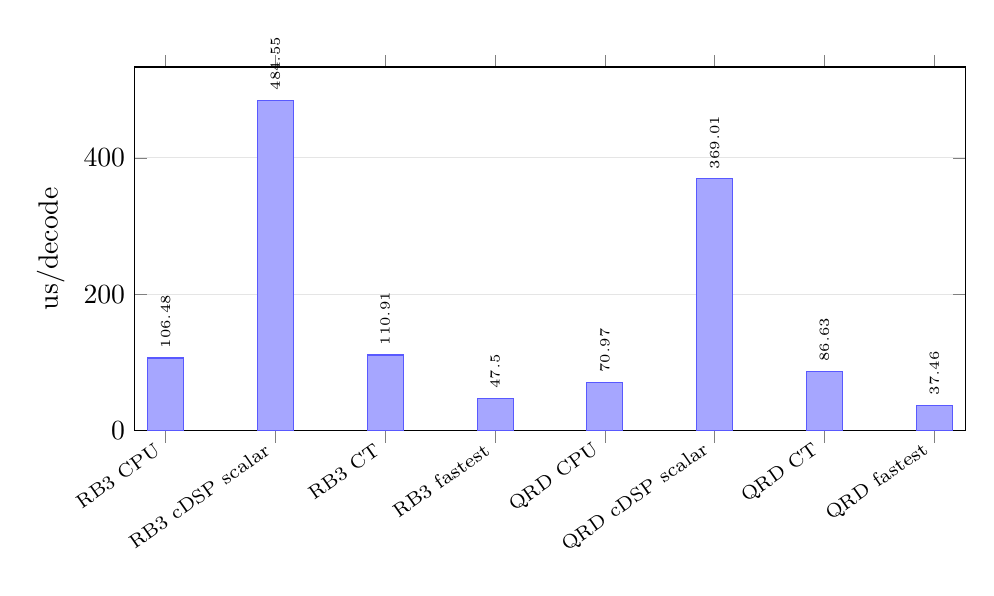
\begin{tikzpicture}
\begin{axis}[
    ybar,
    width=\linewidth,
    height=6.2cm,
    bar width=13pt,
    ymin=0,
    ylabel={us/decode},
    symbolic x coords={RB3 CPU,RB3 cDSP scalar,RB3 CT,RB3 fastest,QRD CPU,QRD cDSP scalar,QRD CT,QRD fastest},
    xtick=data,
    x tick label style={rotate=35, anchor=east, font=\scriptsize},
    nodes near coords,
    every node near coord/.append style={font=\tiny, rotate=90, anchor=west},
    ymajorgrids=true,
    grid style={gray!20},
    enlarge x limits=0.04,
]
\addplot[fill=blue!35, draw=blue!65] coordinates {
    (RB3 CPU,106.479)
    (RB3 cDSP scalar,484.554)
    (RB3 CT,110.908)
    (RB3 fastest,47.495)
    (QRD CPU,70.971)
    (QRD cDSP scalar,369.007)
    (QRD CT,86.633)
    (QRD fastest,37.456)
};
\end{axis}
\end{tikzpicture}
\caption{Real-device decode latency.  Lower is better.}
\label{fig:device-latency}
\end{figure}

\subsection{Discussion}

The simulator results show that the default HVX path reduces HQC-128 decode
cost by 73.5\% relative to scalar while keeping the constant-time-oriented
arithmetic path.  The remaining default CT bottlenecks are RS error-value
computation, Berlekamp--Massey ELP, and RM expand/sum.  The fastest non-CT
path demonstrates the available performance headroom, but it remains
benchmark-only because it uses branchy RS control flow and data-dependent GF/RM
lookup tables.

On physical boards, scalar execution on the ARM64 CPU is faster than the cDSP
scalar FastRPC path.  This means the cDSP only becomes competitive when the HVX
intrinsic kernels are used.  On RB3 Gen 2, the cDSP default CT path is close to
CPU scalar latency, while the fastest non-CT path reaches 47.495 us/decode.  On
QRD8650, the cDSP default CT path reaches 86.633 us/decode and the fastest
non-CT path reaches 37.456 us/decode.





\bibliographystyle{abbrv}
\bibliography{abbrev0,crypto}


\section{Appendix}
\input{appendix/Algorithms}
% \begin{algorithm}[h]
% \caption{HVX-based Hadamard transform}
% \label{alg:hadamard-hvx}
% \begin{algorithmic}[1]
% \Require Input buffer $\mathsf{src}$ containing $128$ signed 16-bit values
% \Require Temporary buffer $\mathsf{dst}$ containing $128$ signed 16-bit values
% \Ensure Hadamard-transformed values are stored in the buffer pointed to by $p_1$

% \State $p_1 \gets \mathsf{src}$
% \State $p_2 \gets \mathsf{dst}$

% \For{$\mathsf{pass} \gets 0$ \textbf{to} $6$}
%     \State $\mathbf{lo} \gets p_1[0:63]$
%     \State $\mathbf{hi} \gets p_1[64:127]$

%     \State $(\mathbf{d}_{lo},\mathbf{d}_{hi}) \gets
%     \mathsf{VDEAL}(\mathbf{hi},\mathbf{lo},2)$

%     \State $\mathbf{v}_e \gets \mathsf{VDEALH}(\mathbf{d}_{lo})$
%     \State $\mathbf{v}_o \gets \mathsf{VDEALH}(\mathbf{d}_{hi})$

%     \State $(\mathbf{sum},\mathbf{diff}) \gets
%     \mathsf{VBFLY}(\mathbf{v}_e,\mathbf{v}_o)$

%     \State $p_2[0:63] \gets \mathbf{sum}$
%     \State $p_2[64:127] \gets \mathbf{diff}$

%     \State $\mathsf{swap}(p_1,p_2)$
% \EndFor

% \State \Return $p_1$
% \end{algorithmic}
% \end{algorithm}


% \begin{algorithm}[h]
% \caption{HVX-based peak detection}
% \label{alg:find-peaks-hvx}
% \begin{algorithmic}[1]
% \Require \parbox[t]{0.82\linewidth}{
% Hadamard-transformed buffer $\mathsf{transform}$ containing $128$ signed
% 16-bit values.
% }
% \Ensure \parbox[t]{0.82\linewidth}{
% Encoded peak position used for Reed-Muller decoding.
% }

% \State $\mathbf{row}_0 \gets \mathsf{transform}[0:63]$
% \State $\mathbf{row}_1 \gets \mathsf{transform}[64:127]$

% \State $\mathbf{abs}_0 \gets \mathsf{VABS}(\mathbf{row}_0)$
% \State $\mathbf{abs}_1 \gets \mathsf{VABS}(\mathbf{row}_1)$

% \State $\mathbf{max} \gets \mathsf{VMAX}(\mathbf{abs}_0,\mathbf{abs}_1)$

% \For{$s \in \{64,32,16,8,4,2\}$}
%     \State $\mathbf{max} \gets
%     \mathsf{VMAX}(\mathbf{max},\mathsf{VROT}_{s}(\mathbf{max}))$
% \EndFor

% \State $a^{*} \gets \mathbf{max}[0]$
% \State $\mathbf{target} \gets \mathsf{VSPLAT}(a^{*})$
% \State $\mathbf{sentinel} \gets \mathsf{VSPLAT}(0x7fff)$

% \State $\mathbf{idx}_0 \gets \mathsf{rm\_index\_lo}$
% \State $\mathbf{idx}_1 \gets \mathsf{rm\_index\_hi}$

% \State $\mathbf{mask}_0 \gets \mathsf{VCMPEQ}(\mathbf{abs}_0,\mathbf{target})$
% \State $\mathbf{mask}_1 \gets \mathsf{VCMPEQ}(\mathbf{abs}_1,\mathbf{target})$

% \State $\mathbf{pos}_0 \gets
% \mathsf{VSELECT}(\mathbf{mask}_0,\mathbf{idx}_0,\mathbf{sentinel})$
% \State $\mathbf{pos}_1 \gets
% \mathsf{VSELECT}(\mathbf{mask}_1,\mathbf{idx}_1,\mathbf{sentinel})$

% \State $\mathbf{peak} \gets \mathsf{VMIN}(\mathbf{pos}_0,\mathbf{pos}_1)$

% \For{$s \in \{64,32,16,8,4,2\}$}
%     \State $\mathbf{peak} \gets
%     \mathsf{VMIN}(\mathbf{peak},\mathsf{VROT}_{s}(\mathbf{peak}))$
% \EndFor

% \State $i^{*} \gets \mathbf{peak}[0]$
% \State $v^{*} \gets \mathsf{transform}[i^{*}]$

% \If{$v^{*} > 0$}
%     \State $i^{*} \gets i^{*} \;|\; 128$
% \EndIf

% \State \Return $i^{*}$
% \end{algorithmic}
% \end{algorithm}

\end{document}
